% debut d'un fichier latex standard
\documentclass[a4paper,12pt,twoside]{article}

% Pour les unités SI
\usepackage{siunitx}
% pour l'inclusion de figures en eps,pdf,jpg
\usepackage{graphicx}
% quelques symboles mathematiques en plus
\usepackage{amsmath}
% le tout en langue francaise
%\usepackage[english]{babel}
% on peut ecrire directement les caracteres avec l'accent
% a utiliser sur Linux/Windows
\usepackage[utf8]{inputenc}
\usepackage[T1]{fontenc}

% pour faire des systèmes d'équations
\usepackage{systeme}

% a utiliser sur le Mac
%\usepackage[applemac]{inputenc}
% pour l'inclusion de links dans le document
\usepackage[colorlinks,bookmarks=false,linkcolor=blue,urlcolor=blue]{hyperref}
\usepackage{subcaption}
\paperheight=297mm
\paperwidth=210mm

\setlength{\textheight}{235mm}
\setlength{\topmargin}{-1.2cm} % pour centrer la page verticalement
%\setlength{\footskip}{5mm}
\setlength{\textwidth}{15cm}
\setlength{\oddsidemargin}{0.56cm}
\setlength{\evensidemargin}{0.56cm}

\pagestyle{plain}

% quelques abreviations utiles
\def \be {\begin{equation}}
\def \ee {\end{equation}}
\def \dd  {{\rm d}}

\newcommand{\mail}[1]{{\href{mailto:#1}{#1}}}
\newcommand{\ftplink}[1]{{\href{ftp://#1}{#1}}}
%
% latex SqueletteRapport.tex      % compile la source LaTeX
% xdvi SqueletteRapport.dvi &     % visualise le resultat
% dvips -t a4 -o SqueletteRapport.ps SqueletteRapport % produit un PostScript
% ps2pdf SqueletteRapport.ps      % convertit en pdf

% pdflatex SqueletteRapport.pdf    % compile et produit un pdf

% ======= Le document commence ici ======

\begin{document}
% Le titre, l'auteur et la date
\title{Particle in an electromagnetic field\\{\small Physique Numérique I}\\{\small 2nd report}}
\date{\today}
\author{Delphine Martres and Damien Korber\\{\small \mail{delphine.martres@epfl.ch} and \mail{damien.korber@epfl.ch}}}
\maketitle
\tableofcontents % Table des matieres

% Quelques options pour les espacements entre lignes, l'identation
% des nouveaux paragraphes, et l'espacement entre paragraphes
\baselineskip=16pt
\parindent=15pt
\parskip=5pt



%%%% ON COMMENCE A ECRIRE D'ICI

\section{Introduction}
A charged elementary particle in an electromagnetic field, such as a proton, is subjected to the Lorentz force $\vec{F}=q(\vec{E} + \vec{v} \times \vec{B})$.
This report will focus on studying how such a particle behaves under the influence of that force, with varying electrical and magnetic fields.

\section{Analytical computations}
\subsection{Establishment of the differential equation system}
The first important step to simulate this problem, is to establish the differential equations.
By considering Newton's second law and Lorentz force, and after some computations that can be found in appendix \ref{ann:dev-eq-diff}, the system of equations \ref{eq:equa-diff} results:

\begin{equation}
\systeme*{m\ddot{x} = Bq\dot{y}, m\ddot{y} = qE - Bq\dot{x}}
\label{eq:equa-diff}
\end{equation}

The equation on $z$ axis is neglected because no information can be obtained from it, as the trajectory is two-dimensional.

\subsection{Analytical solutions with a null electric field}
To compare the numerical results with the analytical results, the solution of the differential system \ref{eq:equa-diff} needs to be found.
To solve it, two simplifications are made: the norm of the electric field $E=0$, and the norm of the magnetic field $B=B_0$, where $B_0$ is constant, which gives to equations \ref{eq:equa-diff-simple}.

\begin{equation}
\systeme*{m\ddot{x} = B_0q\dot{y}, m\ddot{y} = - B_0q\dot{x}}
\label{eq:equa-diff-simple}
\end{equation}

After some computations available in appendix \ref{ann:dev-sol-ana}, the system of equations \ref{eq:sol-ana} results.

\begin{equation}
	\begin{pmatrix} v_x\\ v_y\\ 0\\ \end{pmatrix} = \begin{pmatrix} Acos(\frac{qB_0}{m} t + \phi_x)\\ -Asin(\frac{qB_0}{m} t + \phi_x)\\ 0\\ \end{pmatrix}
\label{eq:sol-ana}
\end{equation}

\subsection{Solution with set initial conditions}

We set $\omega = \frac{qB_0}{m}$. For $v_x=0$ and $v_{y0} = v_0$, equation \ref{eq:sol-v} results.

\begin{equation}
	\begin{pmatrix} v_x\\ v_y\\ 0\\ \end{pmatrix} = \begin{pmatrix} v_0 sin(\omega t)\\ -v_0 cos(\omega t)\\ 0\\ \end{pmatrix}
\label{eq:sol-v}
\end{equation}

And for a trajectory centered on $(0,0)$, we get equation \ref{eq:sol-r}.
\begin{equation}
	\begin{pmatrix} x\\ y\\ 0\\ \end{pmatrix} = \begin{pmatrix} -\frac{v_0}{\omega} cos(\omega t)\\ -\frac{v_0}{\omega} sin(\omega t)\\ 0\\ \end{pmatrix}
\label{eq:sol-r}
\end{equation}
with the initial position \ref{eq:init}.
\begin{equation}
	\begin{pmatrix} x_0\\ y_0\\ 0\\ \end{pmatrix} = \begin{pmatrix} -\frac{v_0}{\omega}\\ 0\\ 0\\ \end{pmatrix}
\label{eq:init}
\end{equation}

All the developments are available in appendix \ref{ann:dev-sol-ana}.

\section{Study of three numerical methods}\label{sec:etudes-integrateur}
The goal of this experiment is to study and compare three numerical methods: Euler, Euler-Cromer and Runge-Kutta of 2nd order, by studying their convergence and their stability through multiple simulations.
In this section, the electric field is $E = 0$.
\subsection{Trajectory, speed, energy and stability}
In this experiment, the initial vertical velocity is equal to $v_0 = \SI{4d5}{\meter\per\second}$ and the constant magnetic field is $B_0 = \SI{3}{\tesla}$.
The simulation stops after the proton has done five revolutions.

\begin{figure}[h]
	\centering
	\begin{subfigure}[t]{0.45\textwidth}
	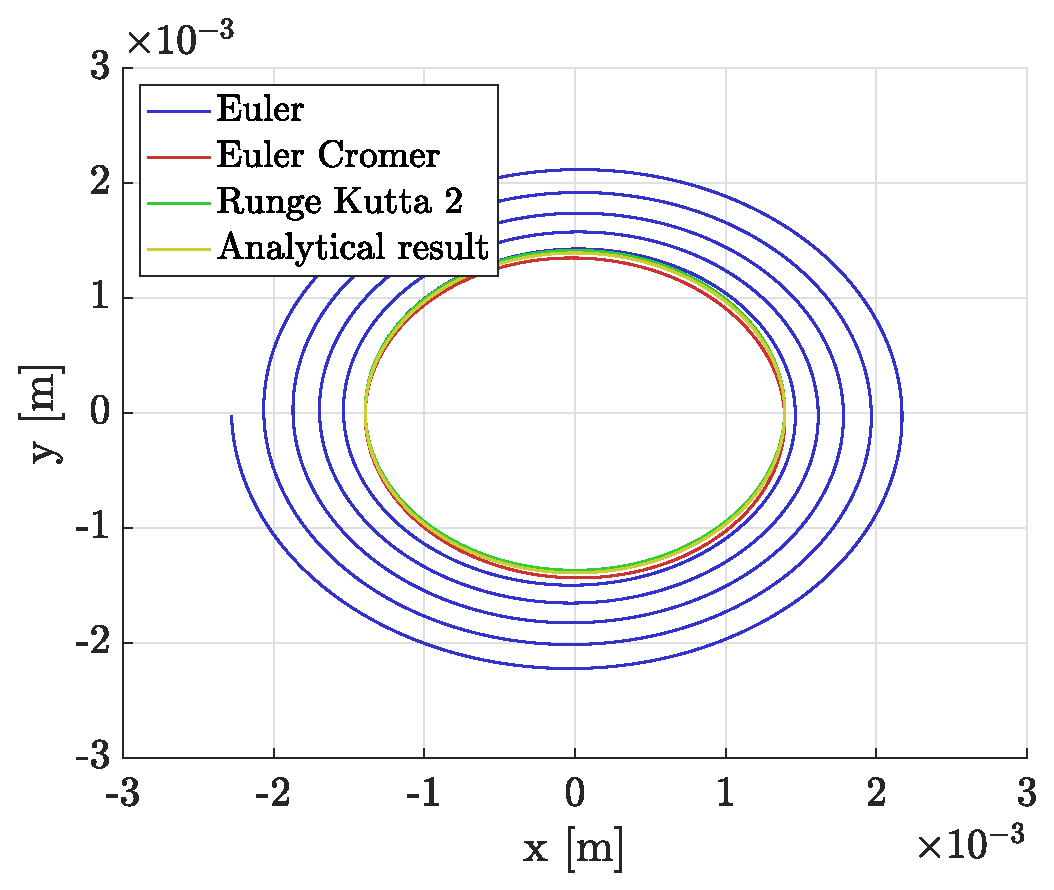
\includegraphics[width=\linewidth]{graphs/ex2_ii_traj_ALL.eps}
		\caption{Trajectory of the proton from three numerical methods and the analytical result.}
		\label{fig:ex2-ii-traj-all}
	\end{subfigure}
	~
	\begin{subfigure}[t]{0.45\textwidth}
		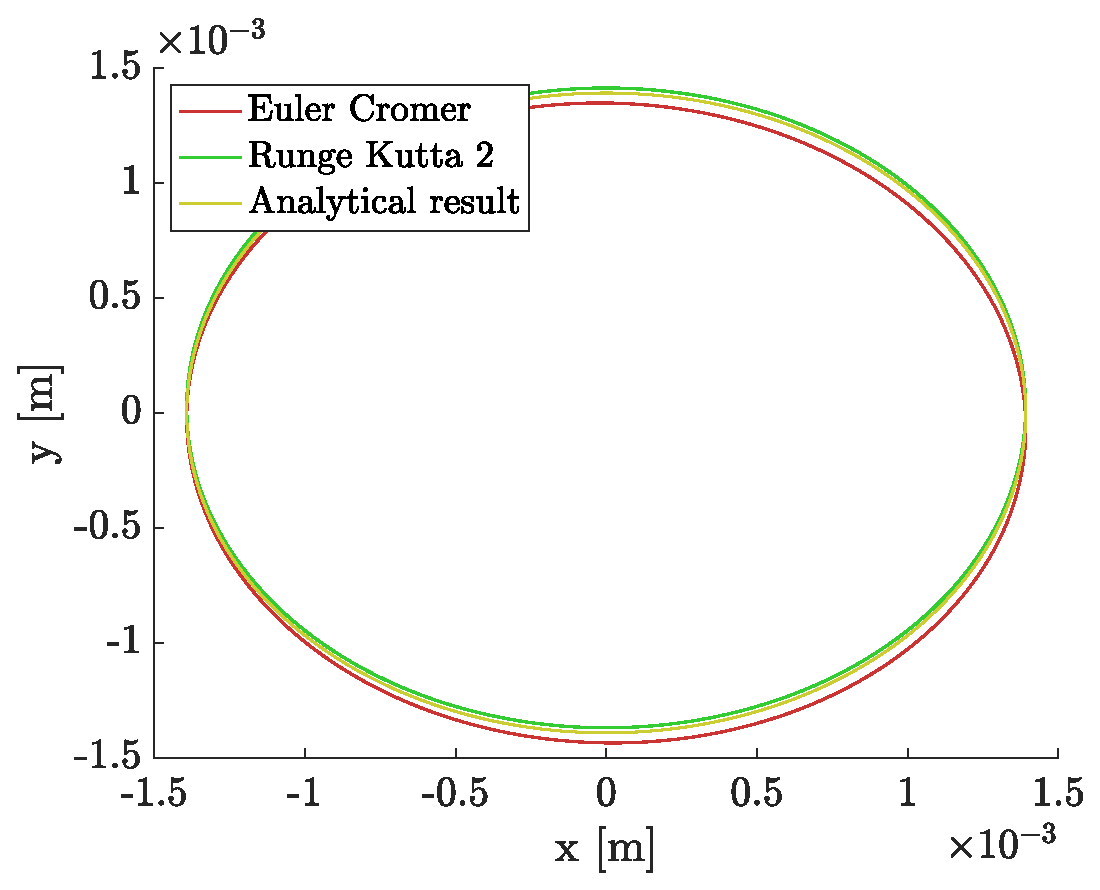
\includegraphics[width=\linewidth]{graphs/ex2_ii_traj_NoEuler}
		\caption{Trajectory of the proton from two numerical methods and the analytical result. Euler's method has being removed to improve clarity of the graph.}
		\label{fig:ex2-ii-traj-NoEuler}
	\end{subfigure}

	\caption{Comparison of the trajectories of the proton using different numericals methods with \num{1000} steps.}
	\label{fig:ex2-ii-traj}
\end{figure}

The main point to notice on figure \ref{fig:ex2-ii-traj-all} is the unsuitability of Euler's method in this experiment.
Indeed, with this method, the proton seems to follow a spiraling trajectory.
As it is only subjected to a uniform magnetic field, the proton is supposed to follow a circular trajectory with a constant radius.
This problem comes directly from the idea of Euler's method itself.
When it evaluates the next iteration, it follows  the tangent of the trajectory, which causes errors to accumulate over each iteration.
The Euler method has the advantages of being easy to implement and not needing a lot of resources to run, but is unsuitable for this problem.\\

Figure \ref{fig:ex2-ii-traj-NoEuler} is better to analyse the two others numerical methods, as Euler's is removed.
In this figure, Euler-Cromer method approximates the trajectory quite well.
It is not perfect as there is still a gap with the analytical solution, but it seems to converge fast enough to be suitable in this problem.
More informations about convergence of this method is done in section \ref{sec:etude-conv}.\\

Still on figure \ref{fig:ex2-ii-traj-NoEuler}, Runge-Kutta of second order seems to be the most suitable out of the numerical methods that were tried in this experiment.
The results are even closer to the analytical solution than Euler-Cromer.

\begin{figure}[h]
	\centering
	\begin{subfigure}[t]{0.45\textwidth}
	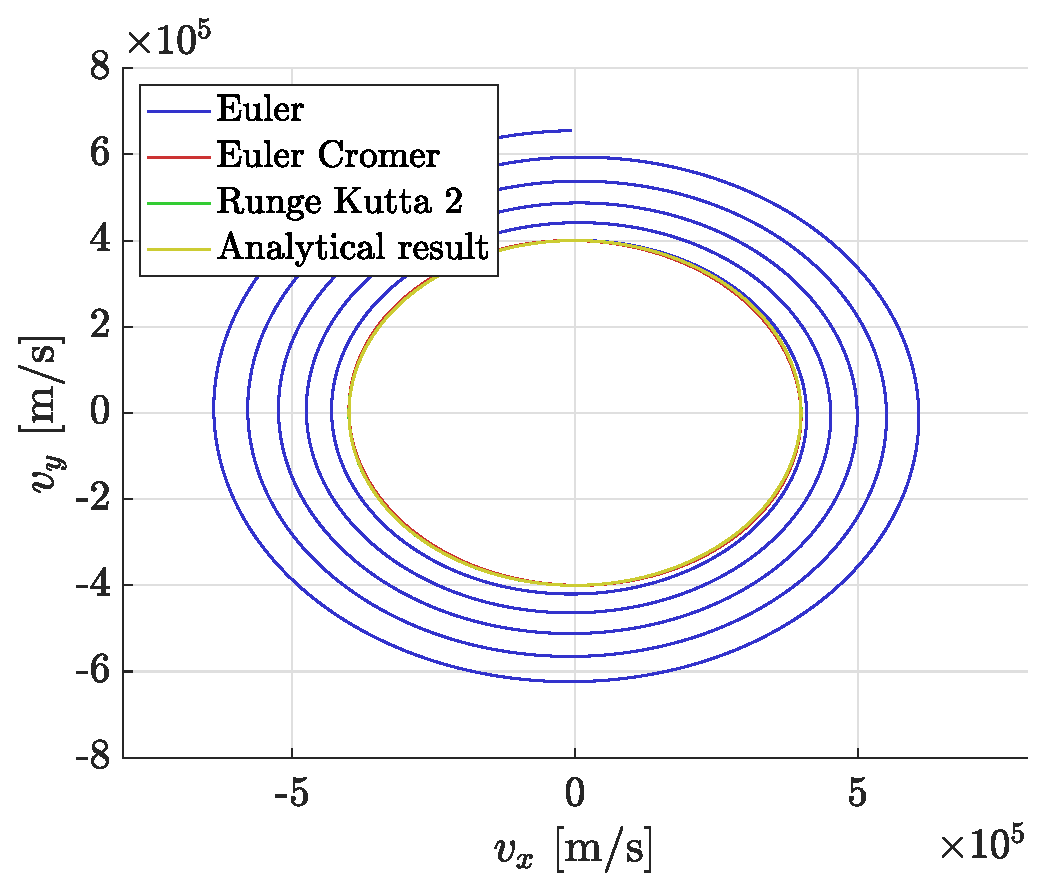
\includegraphics[width=\linewidth]{graphs/ex2_iii_speed_ALL.eps}
		\caption{Orbit of the speed of the proton comparing all numerical methods and the analytical result.}
		\label{fig:ex2-iii-speed-ALL}
	\end{subfigure}
	~
	\begin{subfigure}[t]{0.45\textwidth}
		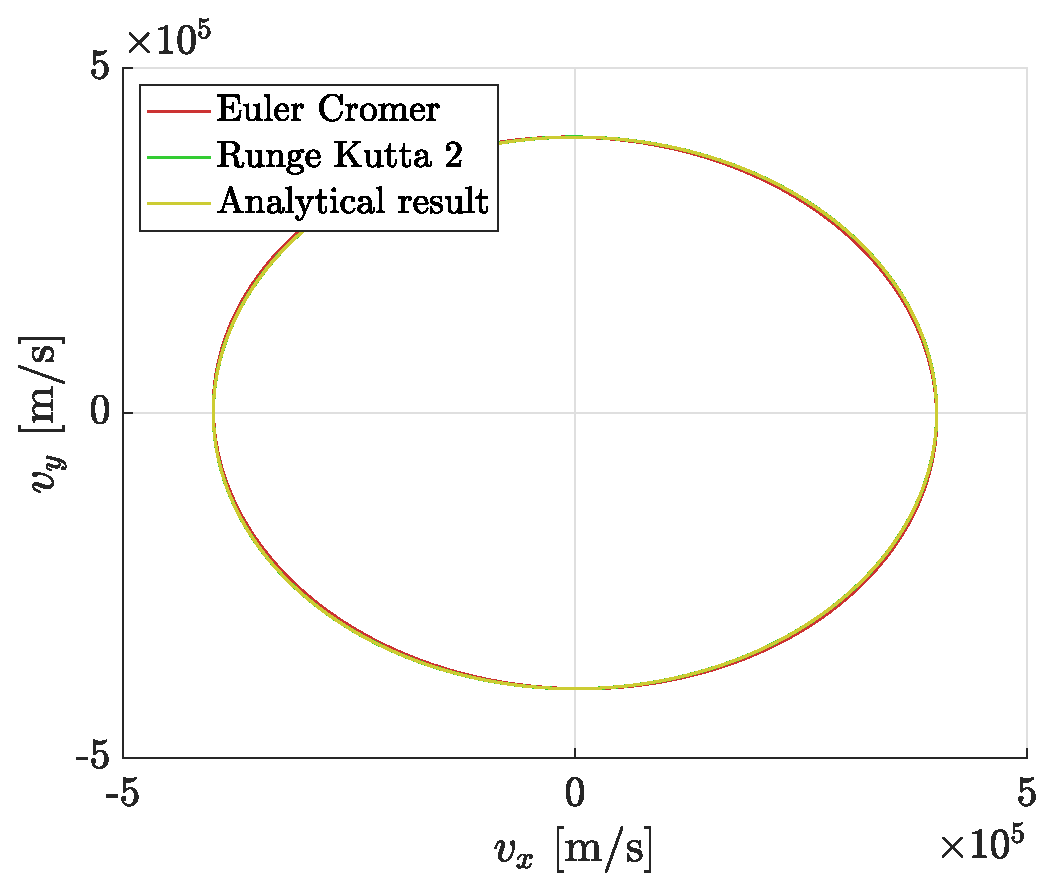
\includegraphics[width=\linewidth]{graphs/ex2_iii_speed_NoEuler.eps}
		\caption{Orbit of the speed of the proton without Euler's method for readability.}
		\label{fig:ex2-iii-speed-NoEuler}
	\end{subfigure}

	\caption{Orbit of the speed of the protons using different numericals methods with \num{1000} steps.} %TODO: Est-ce que le terme 'speed orbit' est bien choisi ?
	\label{fig:ex2-iii-speed}
\end{figure}

The same observations as before can be made about figure \ref{fig:ex2-iii-speed}.
There is not much to say about figure \ref{fig:ex2-iii-speed-ALL}, it is the same analysis as before.
The only notable thing here is the closeness between the analytical solution and the simulation using the Runge-Kutta method.
Figure \ref{fig:ex2-iii-speed-NoEuler} needs to be zoomed into to distinguish a difference between these curves.
Again, for the speed, Runge-Kutta of second order seems better than the other methods.\\

\begin{figure}[h]
\centering
	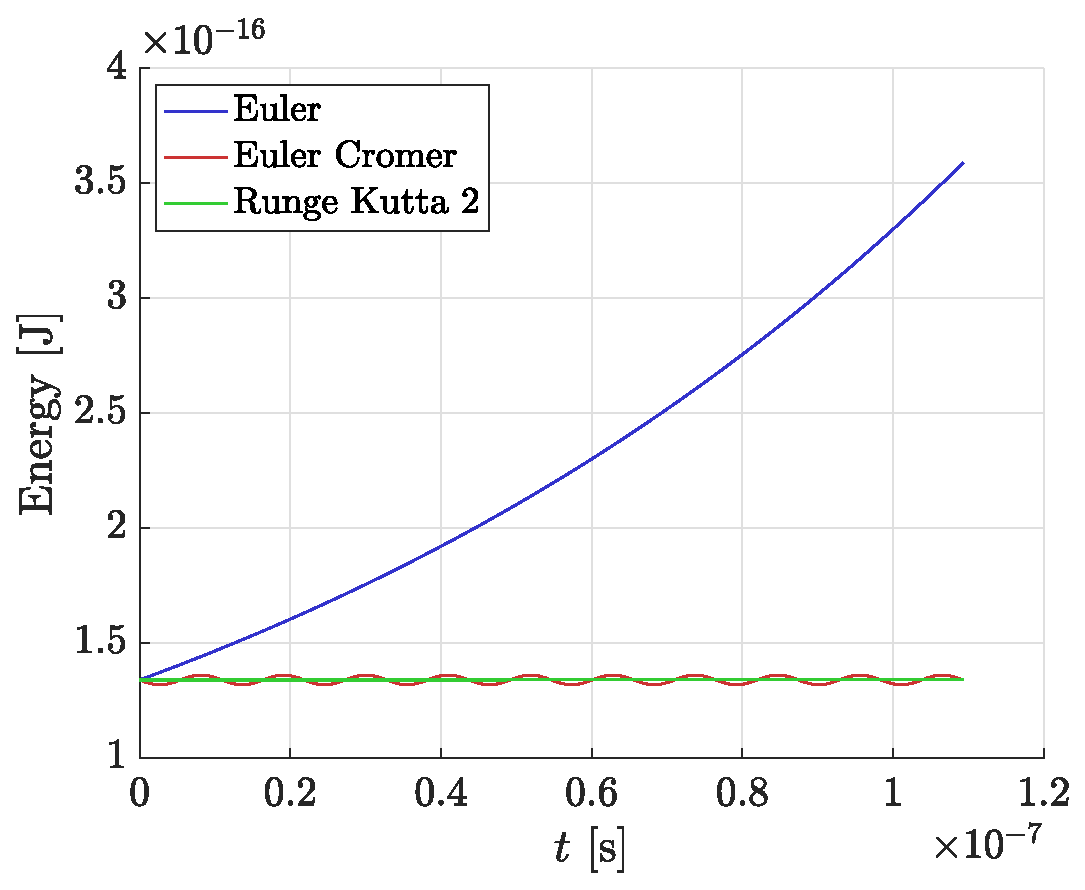
\includegraphics[width=0.6\textwidth]{graphs/ex2_iii_ene.eps}
	\caption{Comparison of mechanical energy of the proton over time, estimated with three different numerical methods for \num{1000} steps.}
	\label{fig:ex2_iii_ene}
\end{figure}

Figure \ref{fig:ex2_iii_ene} is much more interesting than the previous one.
Once again, Euler's method is shown as unsuitable for this experiment.
As time advances, the energy keeps increasing when evaluated by Euler's method, which is impossible because the proton does not receive energy from an external source.
Hence this numerical method is unstable as it does not conserve energy.\\

The energy evaluated with Euler-Cromer has an interesting behaviour: the energy oscillate between two values, and never exceeds these limits.
This comes from the fact that Euler-Cromer is a symplectic method, which means that energy is not conserved, but is bounded.
Properly speaking, this numerical method is not conserving energy over time but limits the error in a certain range, which is enough to get a good approximation of the problem, because the error will not explode as it would using Euler's method.
This also means that the mean energy is conserved.
So with Euler-Cromer's method, energy is not conserved but the method is stable.\\

Finally, there is the energy evaluated by Runge-Kutta of second order.
Energy is conserved over time, which implies the stability of the numerical method.\\



\subsection{Convergence study}\label{sec:etude-conv}
One important part of part of any analysis of a simulation is the study of convergence of the numerical methods used.
A numerical method converges when the computed solution approaches the theoretical solution the smaller the time step used is.\\

\begin{figure}[h]
\centering
\begin{subfigure}[t]{0.45\textwidth}
	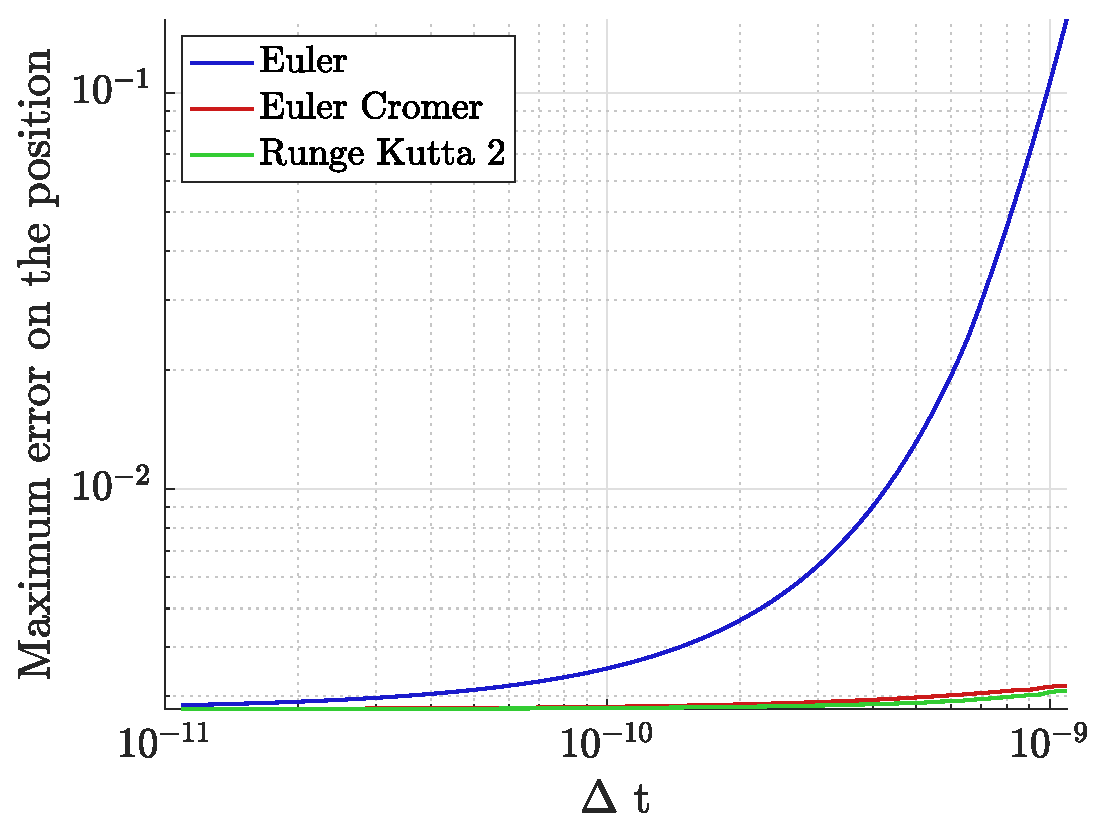
\includegraphics[width=\textwidth]{graphs/ex2_ii_conv_ALL.eps}
	\caption{Convergence graph where three methods are drawn.}
	\label{fig:app1-conv-ALL}
\end{subfigure}
~
\begin{subfigure}[t]{0.45\textwidth}
	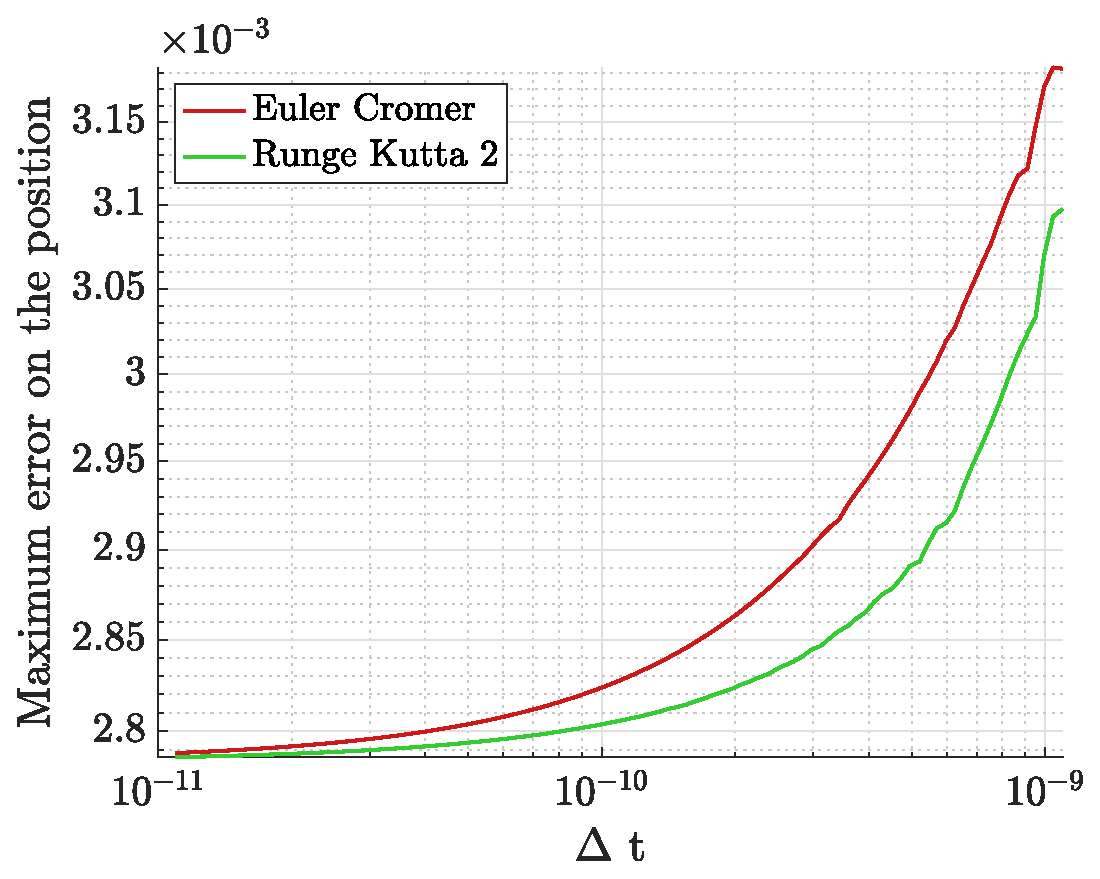
\includegraphics[width=\textwidth]{graphs/ex2_ii_conv_NoEuler.eps}
	\caption{Convergence graph where Euler's method isn't drawn for readability reasons.}
	\label{fig:app1-conv-noEuler}
\end{subfigure}
\caption{Convergence graph comparing Euler, Euler Cromer and Runge Kutta of 2nd order's methods.}
\label{fig:app1-conv}
\end{figure}

On figure \ref{fig:app1-conv-ALL}, all methods seem to converge, but Euler's does so the slowest out of them.
Compared to the two others, Euler needs a really small time step to get a usable approximation of the solution.
This is a problem because it costs a lot of resources to reduce the time step of any simulation.
The real issue with this is the case where the duration of the simulation increases.
This implies a drastic increase of the number of steps evaluated by the methods, as the time step remains constant.
Adding this to fact that the methods needs a small time step in any case, it becomes completely pointless to use it.\\

Figure \ref{fig:app1-conv-noEuler} shows the same convergence study, but focuses on Euler-Cromer and Runge-Kutta's methods.
The main information that can be extracted from this figure is the fact that Runge Kutta of 2nd order converges faster than Euler Cromer.
These methods are appropriate for this project.
A moderate number of steps is enough to get a good approximation of the solution, so both methods seem usable with respect to the convergence.\\

\subsection{Summary}
Section \ref{sec:etudes-integrateur} aims to compare three numerical methods: Euler, Euler-Cromer and Runge-Kutta 2.
In this analysis, two main point are considered: the stability and the convergence of the numerical methods.
Table \ref{tab:comparaison-integrateur} summaries what was learnt about these numerical methods.\\

\begin{table}[h]
\centering
\begin{tabular}{c | c | c | c}
	Numerical method & Does converge ? & Is stable ? & Is energy conserved ? \\
	\hline
	Euler & Yes & No & No\\
	Euler-Cromer & Yes & Yes & No \\
	Runge-Kutta 2 & Yes & Yes & Yes\\
\end{tabular}
\caption{Summary of all three numerical methods}
\label{tab:comparaison-integrateur}
\end{table}

\section{Applications}
\subsection{Drift $\mathbf{E}\times \mathbf{B}$}
In this experiment, the proton is now subjected to an electric field $E=\SI{6d4}{\volt\per\meter}$, as well as a constant magnetic field $B_0 = \SI{3}{\tesla}$.
The proton starts with an initial velocity of $v_{0x}=\SI{0}{\meter\per\second}$ and $v_{0y}=\SI{4d5}{\meter\per\second}$, and the simulation will last the time it takes for the proton to end five revolutions.

\subsubsection{Convergence study}
The first point to study is to check if the Runge-Kutta of 2nd order converges for this experiment.
Figure \ref{fig:app1-i-conv} show a study on the convergence of the position.
In both figure \ref{fig:app1-i-conv-x} and \ref{fig:app1-i-conv-y}, the final position of the simulation clearly approaches a certain point, which implies the convergence of the method.
It also shows that after a certain point, it is not required to use a smaller time step.
In both case, a time step of \SI{d-10}{\second} is close enough to get a good approximation of the solutions, and using a smaller one would only be a waste of resources.

\begin{figure}[h]
\centering
\begin{subfigure}[t]{0.45\textwidth}
	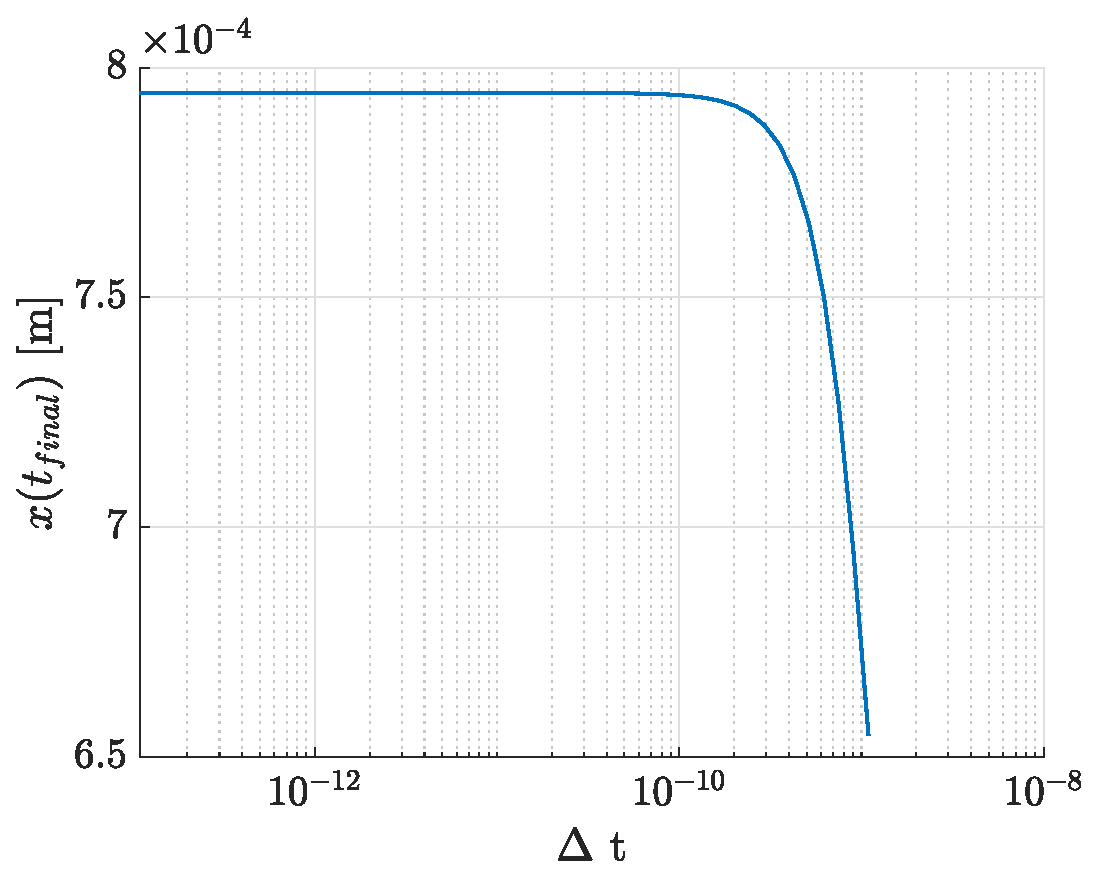
\includegraphics[width=\textwidth]{graphs/app1_i_conv_x.eps}
	\caption{Final horizontal position with respect to the time step.}
	\label{fig:app1-i-conv-x}
\end{subfigure}
~
\begin{subfigure}[t]{0.45\textwidth}
	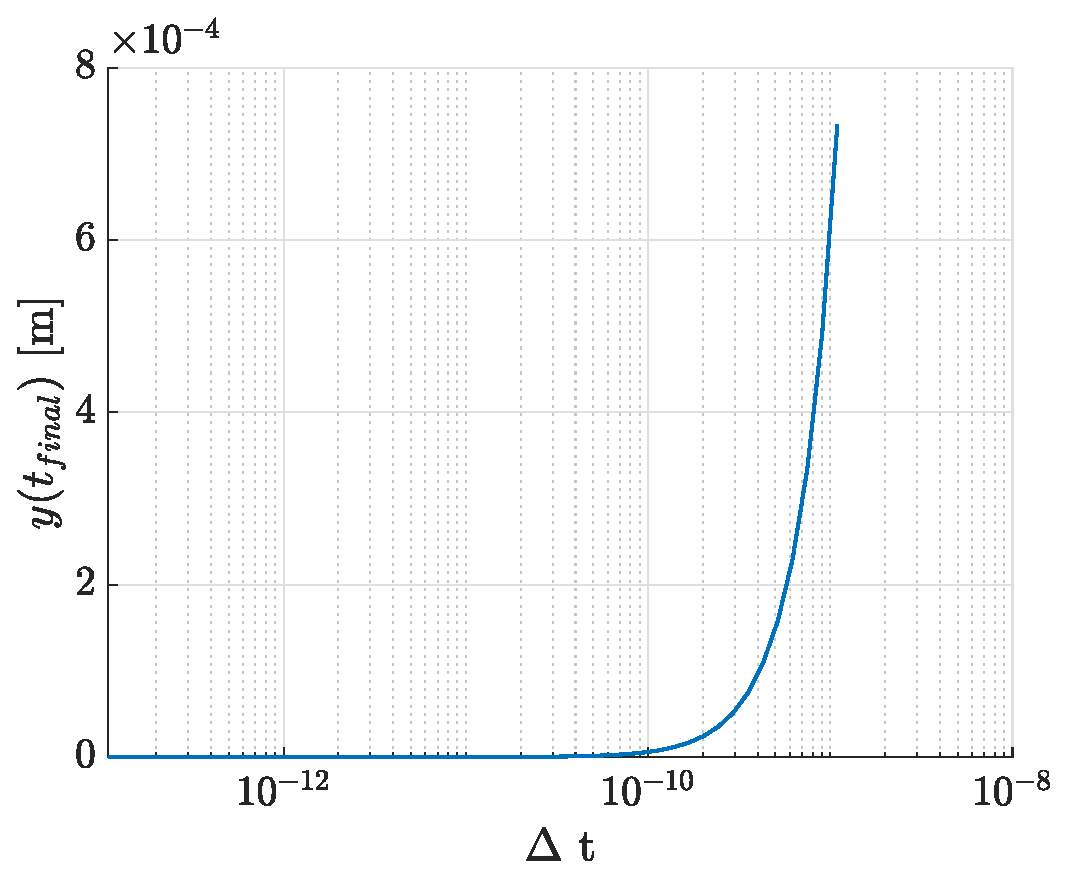
\includegraphics[width=\textwidth]{graphs/app1_i_conv_y.eps}
	\caption{Final vertical position with respect to the time step.}
	\label{fig:app1-i-conv-y}
\end{subfigure}
\caption{Convergence study of the position with respect to the time step using Runge-Kutta of 2nd order.}
\label{fig:app1-i-conv}
\end{figure}


\subsubsection{Energy, trajectory and velocity analysis}
\begin{figure}[h]
\begin{subfigure}[t]{0.32\textwidth}
	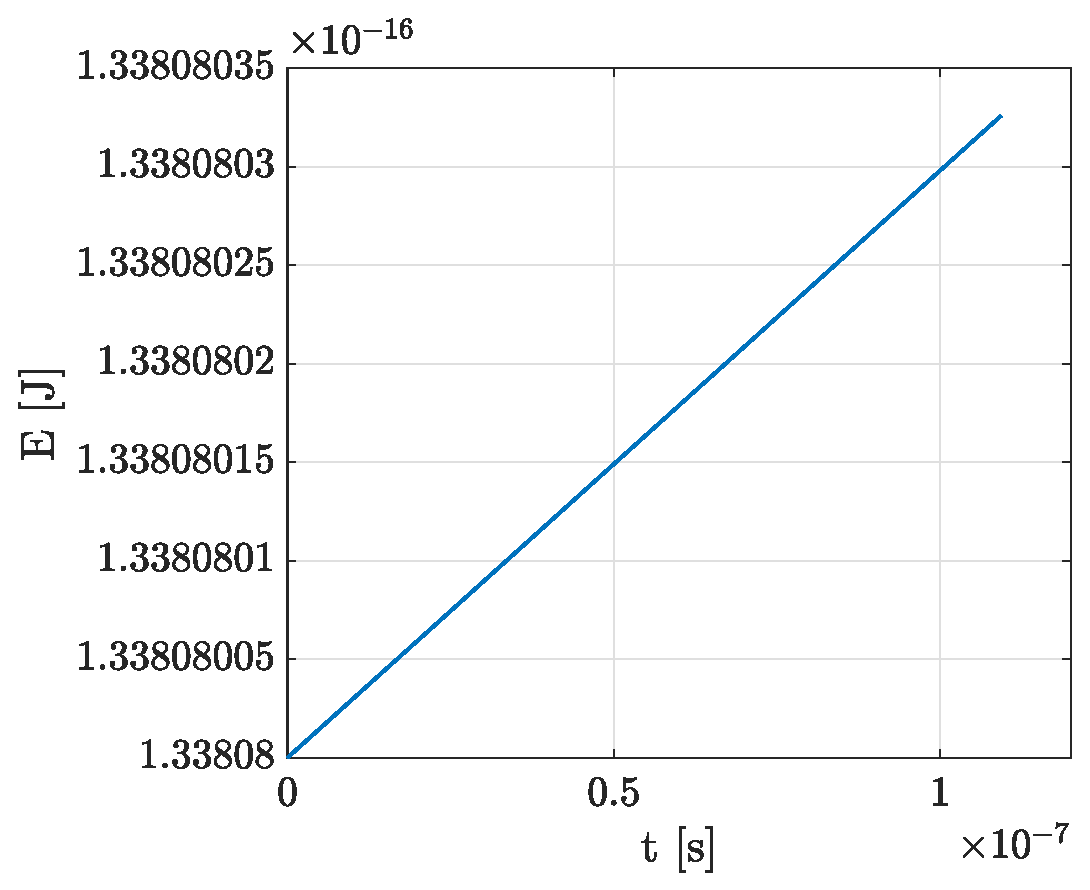
\includegraphics[width=\textwidth]{graphs/app1_ii_ene.eps}
	\caption{Graph showing the energy of the proton over time.}
	\label{fig:app1-ii-ene}
\end{subfigure}
~
\begin{subfigure}[t]{0.32\textwidth}
	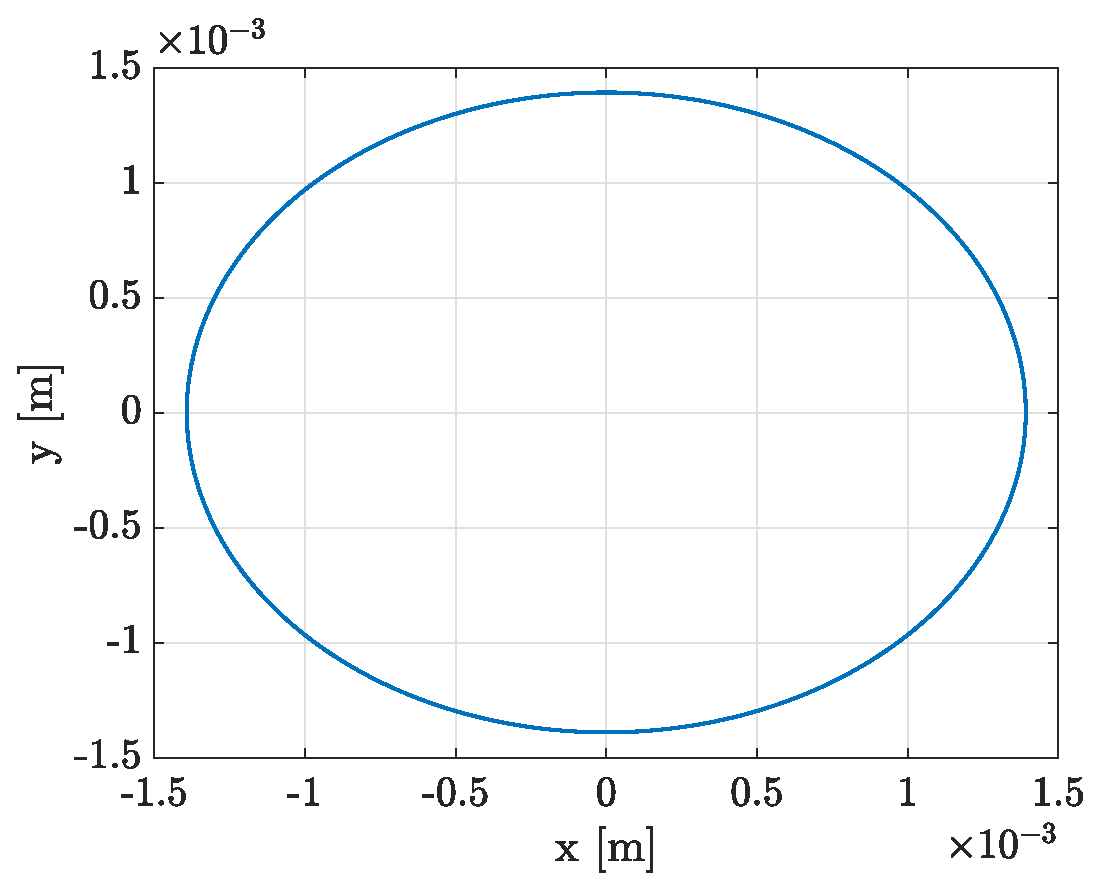
\includegraphics[width=\textwidth]{graphs/app1_ii_traj.eps}
	\caption{Trajectory of the proton.}
	\label{fig:app1-ii-traj}
\end{subfigure}
~
\begin{subfigure}[t]{0.32\textwidth}
	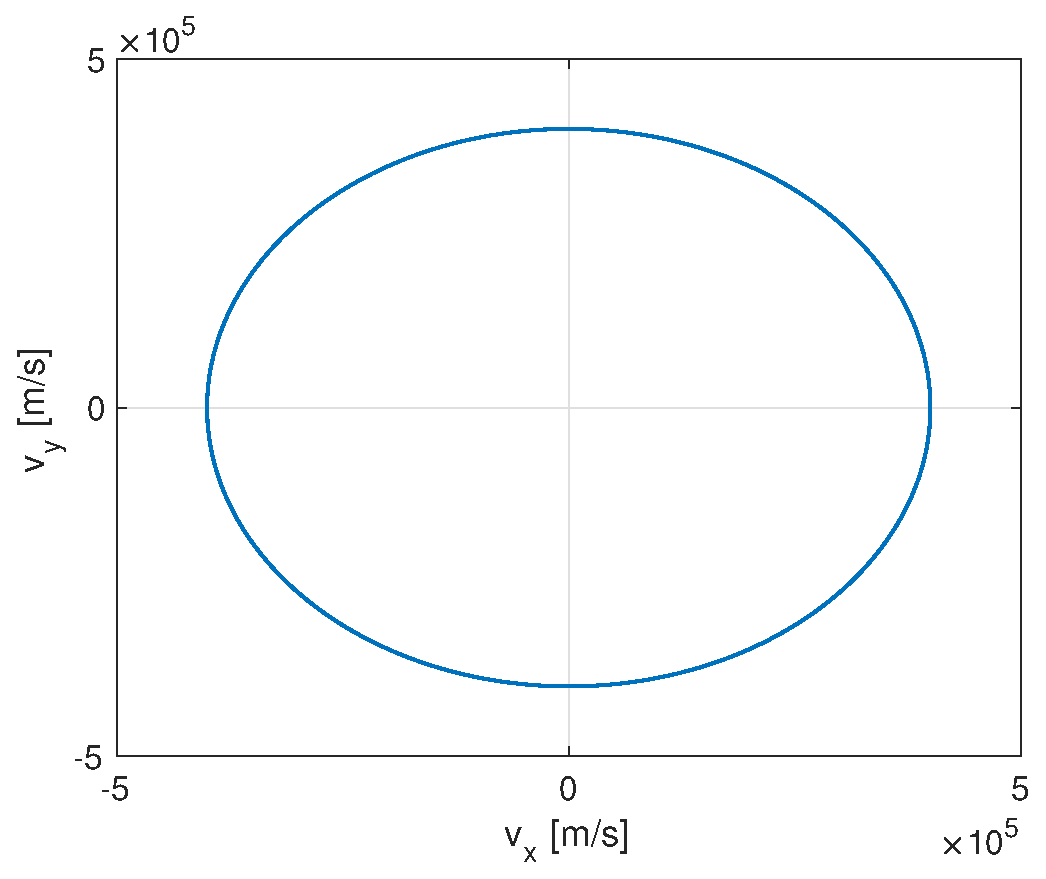
\includegraphics[width=\textwidth]{graphs/app1_ii_vit.eps}
	\caption{Vertical speed in function of horizontal speed of the proton}
	\label{fig:app1-ii-vit}
\end{subfigure}
\caption{Proton in both electric and magnetic fields. The parameter are the ones asked, the integration method is Runge-Kutta of 2nd order, and the number of steps is \SI{1000}{}.}
\label{fig:app1_ii}
\end{figure}

Figure \ref{fig:app1-ii-ene} show the energy of the proton over time.
On first glance, this figure may look odd.
The proton seems to gain energy over time, which is impossible in this context.
However the difference of energy between during the experiment is of order $\SI{d-23}{}$.
This is really small compared to the energy of the proton at any time.
The mean slope is of $\SI{d-16}{}$, which implies an almost horizontal line.
The problem probably comes from the computer itself.
Each time it makes a computation, some results are rounded, which implies that the following computations are not exact, and through time, it accumulates and create a small difference.
Therefore, we can consider energy to be conserved.\\

The figures \ref{fig:app1-ii-traj} and \ref{fig:app1-ii-vit} show the trajectory and the speeds of the proton for the times the proton takes to achieve five revolutions.
The most interesting point to notice is the fact that the trajectory looks like a circle.
All revolutions look stacked, which confirms that the energy is conserved in this experiment.
If it were not, the trajectory would be a spiral.
The same analysis is performed for the second figure.
All revolutions are stacked, the curve looks like a circle, so energy must be conserved.\\

\subsubsection{Proton in a moving frame of reference}
In this experiment, the electric field $E$ is not null anymore.
Its norm is equal to $E=\SI{6d4}{\newton\per\coulomb}$.
Here a different frame of reference is considered.
It uses the same axis as the previous one, but has a velocity expressed by equation \ref{eq:vE}.
\begin{equation}
	v_E = \frac{1}{B^2}\vec{E}\times\vec{B}
	\label{eq:vE}
\end{equation}%TODO: Vérifier l'équation.
Figure \ref{fig:app1_iii_traj} shows the trajectory of the proton when it enters the magnetic and electric field.
The main point of this experiment is to show that changing the frame of reference to a well chosen moving one can nullify all effects of the electric field.
\begin{figure}[h]
\centering
	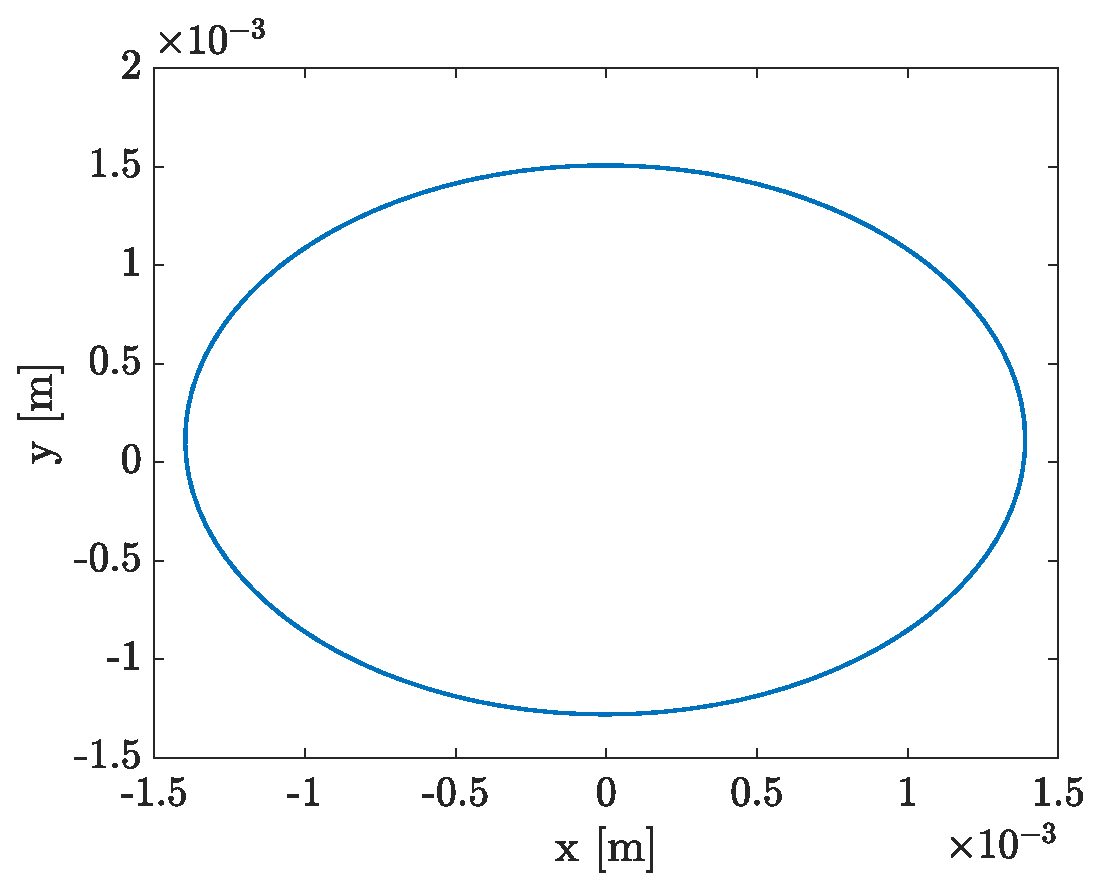
\includegraphics[width=0.6\textwidth]{graphs/app1_iii_traj.eps}
	\caption{Trajectory of the proton in the moving frame of reference. The simulation used \num{1000} steps and Runge-Kutta 2's method. In the legend, the electric field $E$ is expressed in \si{\newton\per\coulomb}, and the velocity $v_E$ is expressed in \si{\meter\per\second}.}
	\label{fig:app1_iii_traj}
\end{figure}

In figure \ref{fig:app1_iii_traj}, both the trajectory of the proton with $E=0$ using the terrestrial reference frame and the one with $E=\num{6d4}$ using the moving reference frame are shown.
A slight difference can be seen between those trajectories, which seems to disprove the previous conjecture.
A possible explanation are numerical errors.
The simulations are not similar and does not use the same values, which probably leads to a divergence.
Another possible explanation is direction of the Lorentz force.
This force is tangential to the trajectory, which implies that, in general, both x and y components of the force are non-null.
This may lead to a slight difference between both trajectories.




\subsection{Drift $\nabla B$}
In this experiment, the particle is now subjected to a magnetic field $\vec{B}=B(x)\hat{z}$, with $B(x)=B_0(1+\kappa x)$, $\kappa=\SI{100}{\metre^{-1}}$, $B_0=3T, E=0, v_{x0}=0$, $v_{y0}=\SI{4d5}{\metre\per\second}$ and over the same period of time as in the first experiment.
All the results are computed using the Runge-Kutta 2 integrator.

\subsubsection{Effect of the magnetic field on a proton and an antiproton}

Simulations are run in the case of a proton, i.e. $q=e$ and in the case of an antiproton, i.e. $q=-e$. For the antiproton, the sign of the initial position $x_0$ is changed.

\begin{figure}[h]
\centering
\begin{subfigure}[t]{0.45\textwidth}
	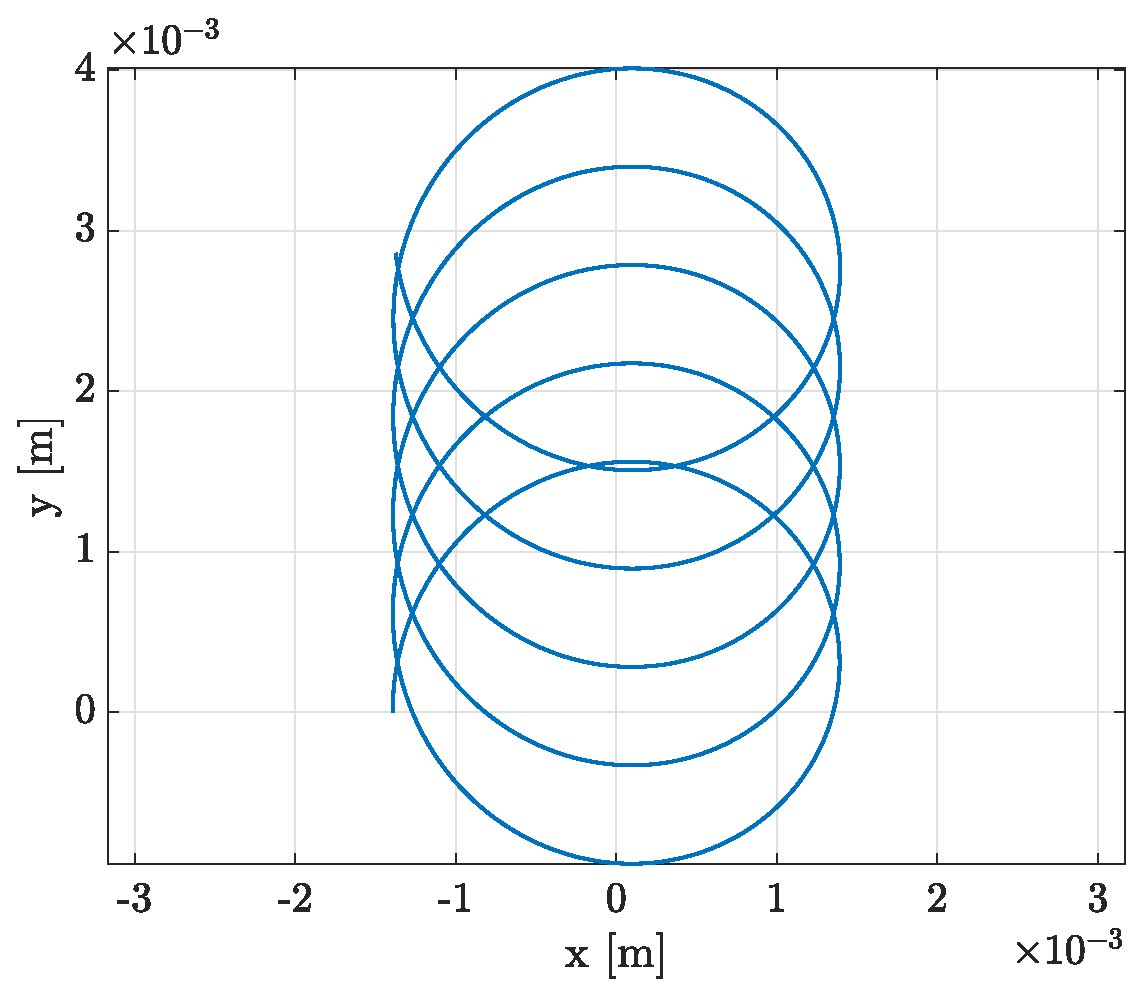
\includegraphics[width=\textwidth]{graphs/app2_ipos_traj.eps}
	\caption{Proton trajectory}
	\label{fig:app2-ipos-traj}
\end{subfigure}
~
\begin{subfigure}[t]{0.45\textwidth}
	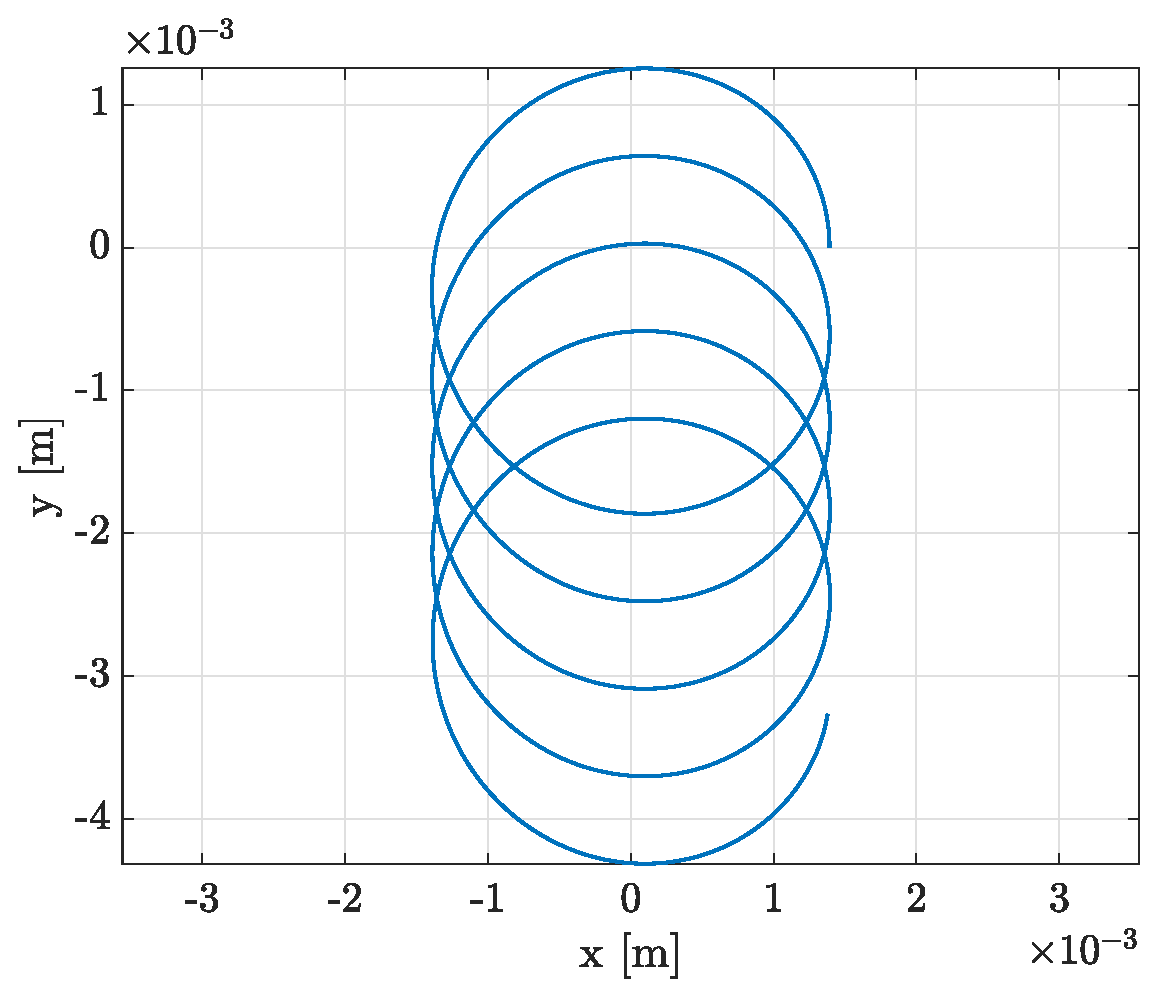
\includegraphics[width=\textwidth]{graphs/app2_ineg_traj.eps}
	\caption{Antiproton trajectory}
	\label{fig:app2-ineg-traj}
\end{subfigure}
\caption{Trajectories of a proton and an antiproton in the magnetic field $\vec{B}$}
\label{fig:app2_i_traj}
\end{figure}

Figure \ref{fig:app2_i_traj} shows the trajectories of both particles in the magnetic field $B$.
In both cases, the particle follows a vertical spiral, in the positive direction of $y$ for the proton and in the negative direction of $y$ for the antiproton. The antiproton also rotates in the opposite direction of the proton (counter-clockwise).

\begin{figure}[h]
\centering
\begin{subfigure}[t]{0.45\textwidth}
	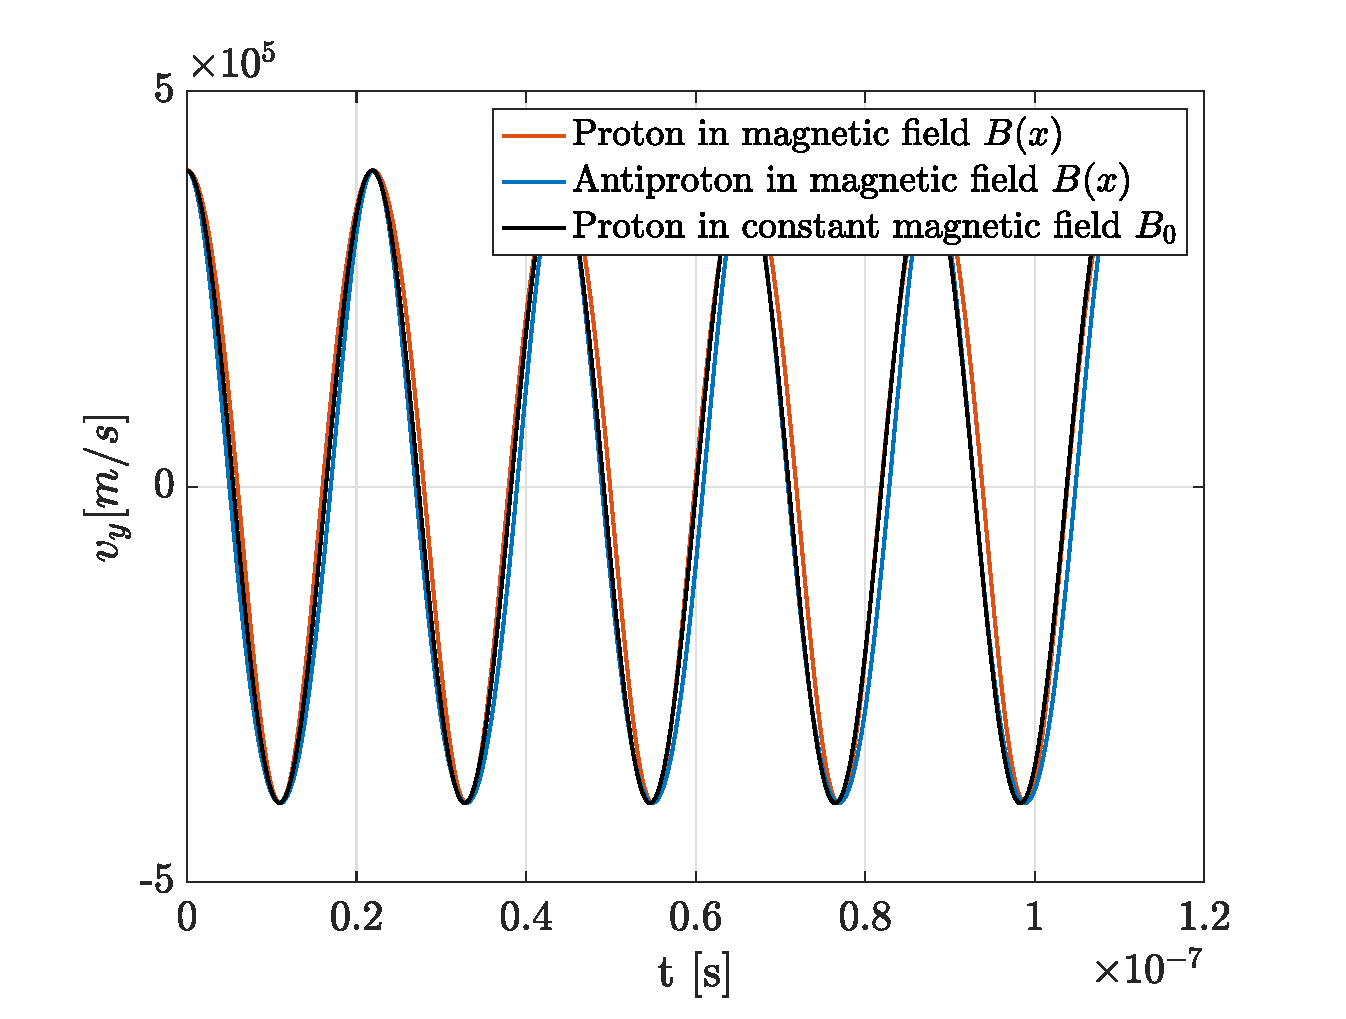
\includegraphics[width=\textwidth]{graphs/app2_i_vyt.eps}
\end{subfigure}
~
\begin{subfigure}[t]{0.48\textwidth}
	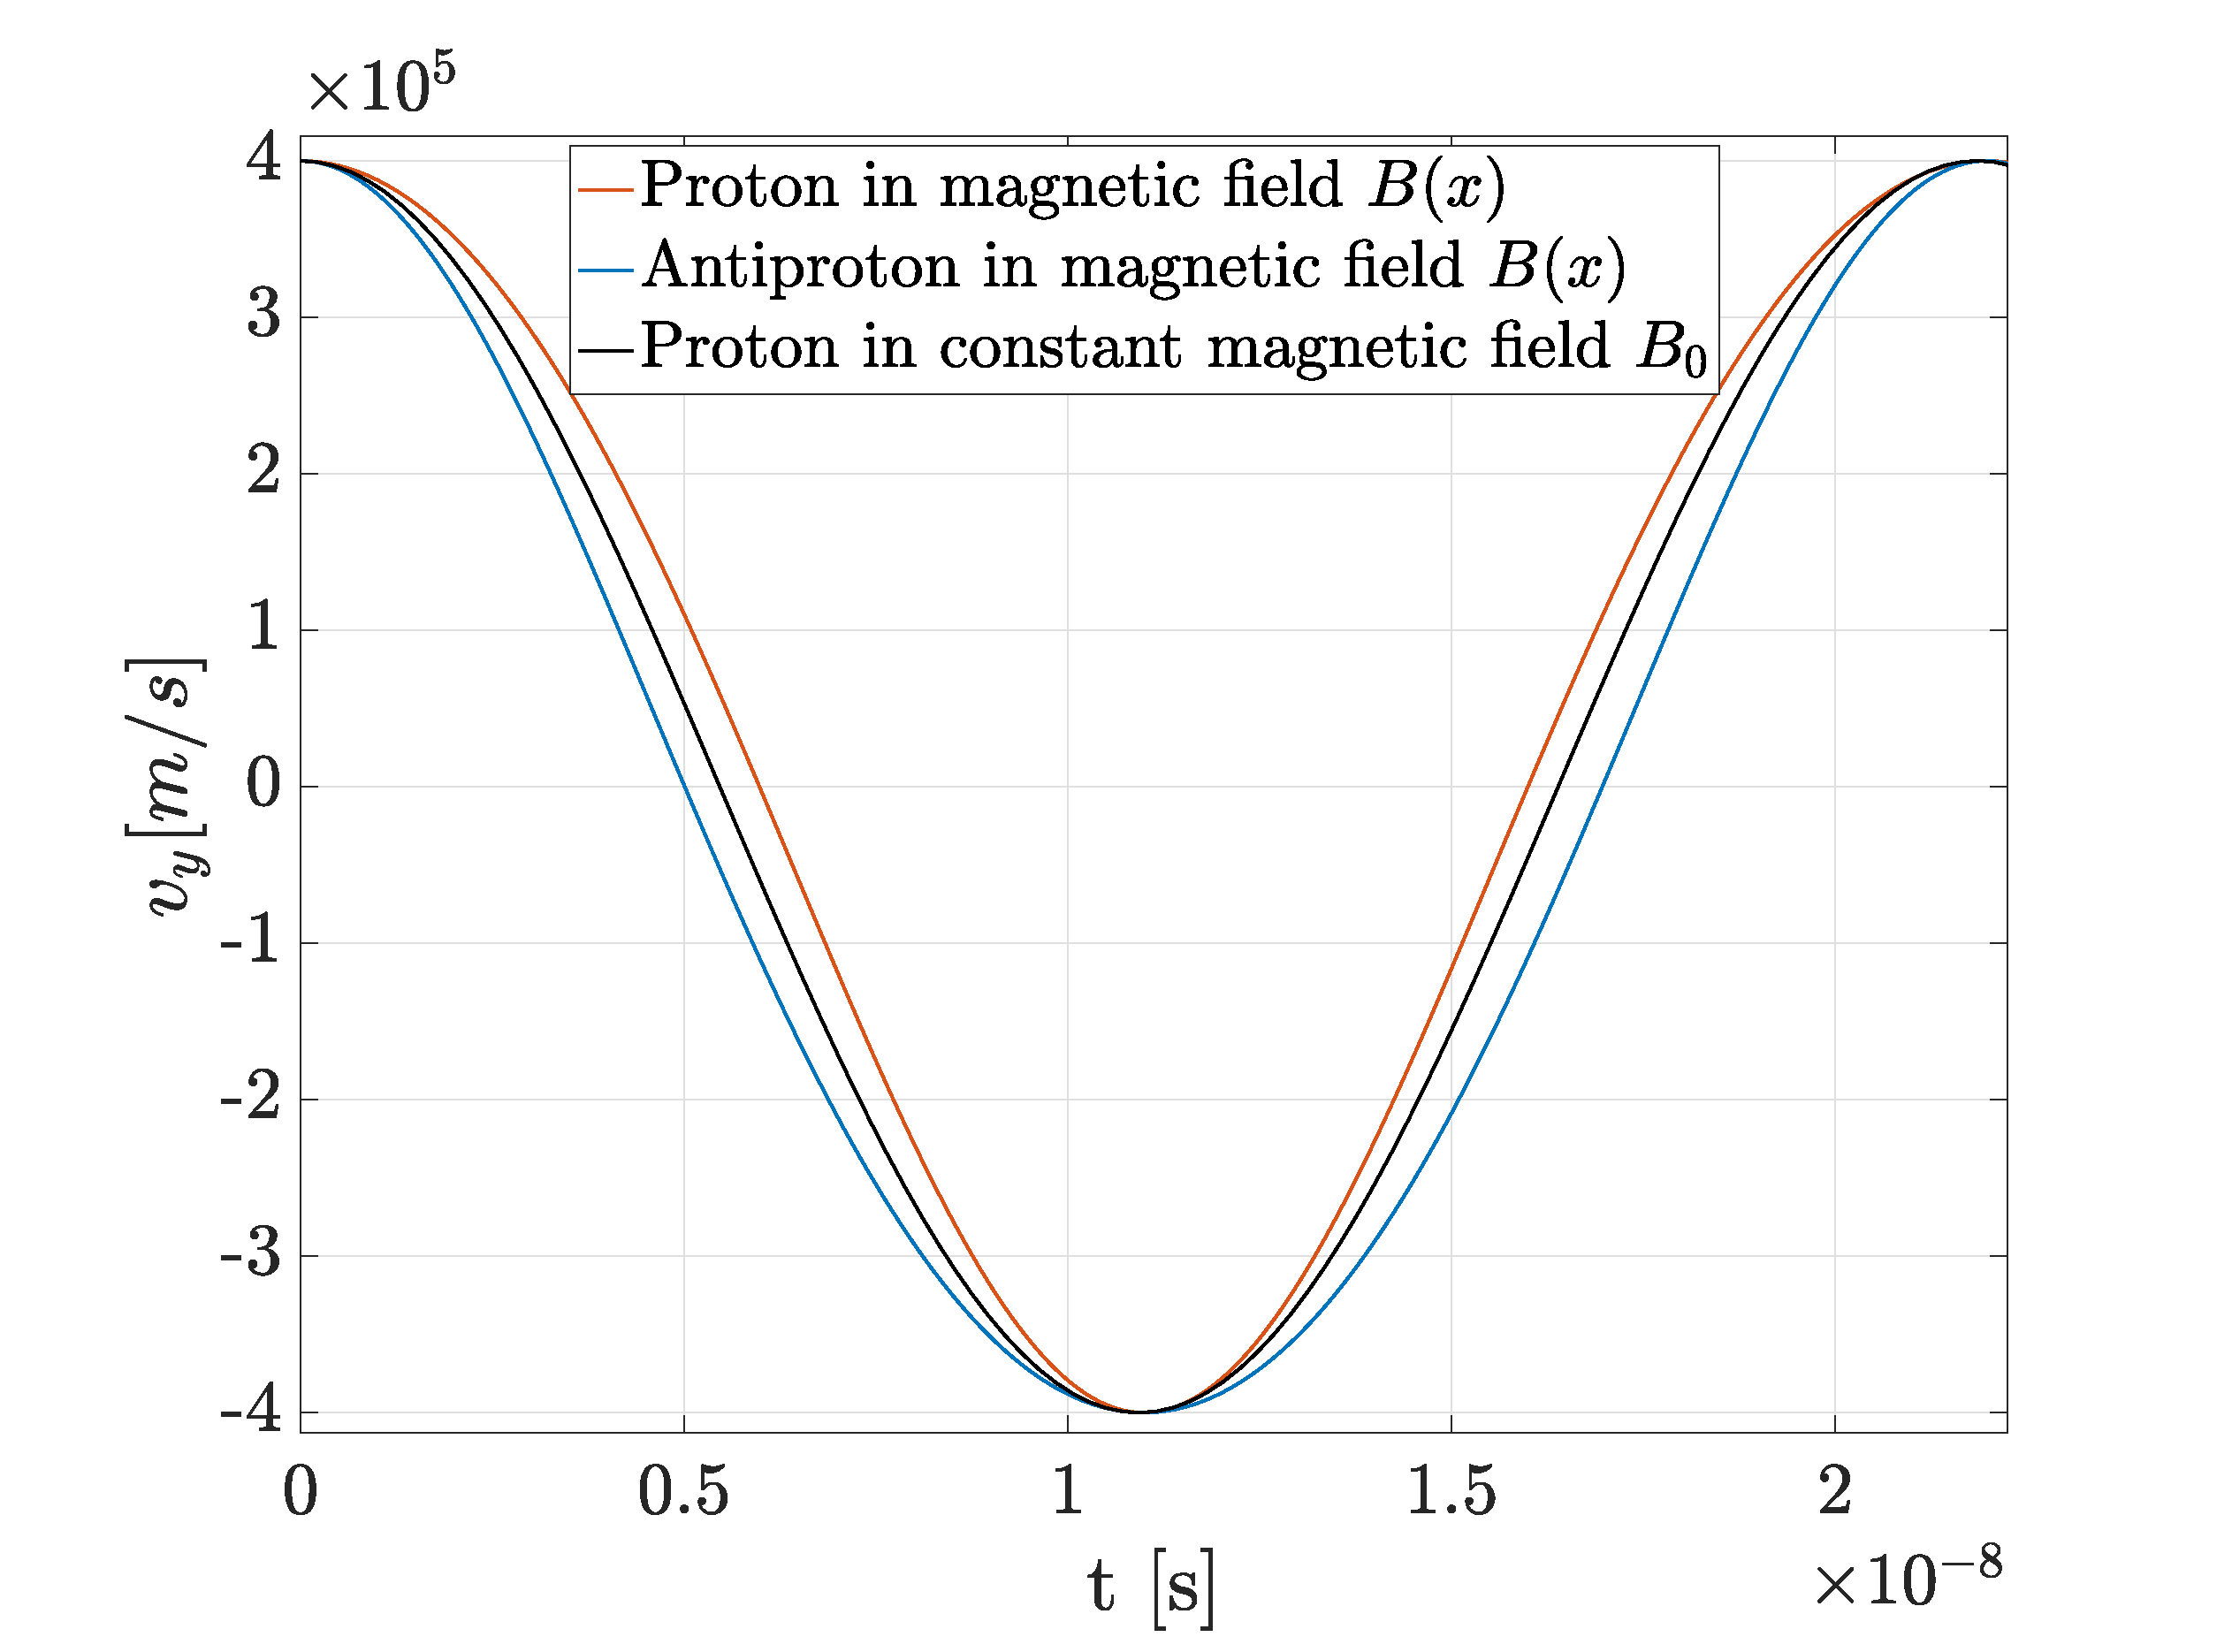
\includegraphics[width=\textwidth]{graphs/vyzoom.eps}
\end{subfigure}
	\caption{Vertical velocity $v_y$ of a proton and an antiproton in the magnetic field $\vec{B}$ and of a proton in the constant magnetic field $B_0\hat{z}$ (zoomed in on the right-hand side graph)}
	\label{fig:app2_i_vyt}
\end{figure}

On figure \ref{fig:app2_i_vyt} the comparison of the vertical velocities of each particle shows that the proton in the variable magnetic field $\vec{B}$ accelerates faster in the positive direction, and slower in the negative direction, than the proton in the constant magnetic field. The opposite is true for the antiproton.

Indeed the expression of the Lorentz force in the variable magnetic field with $E=0$ is:
\begin{equation}
	\vec{F} = q\vec{v} \times \vec{B} = q\vec{v} \times B_0(1+\kappa x)\hat{z}
	\label{mag_force}
\end{equation}
Equation \ref{mag_force} implies that the magnitude of the Lorentz force in a variable magnetic field is also variable. It depends on the horizontal position $x$ of the particle. It is minimal when $x$ is minimal, i.e. at the leftmost point of the quasi-circular trajectory, where $v_y$ is maximal in the positive direction, and it is maximal at its rightmost point, when $x$ is maximal, and $v_y$ is maximal in the negative direction. The force is perpendicular to the velocity $\vec{v}$ in the $xy$ plane, towards the interior of the trajectory.

\begin{figure}[h]
\centering
	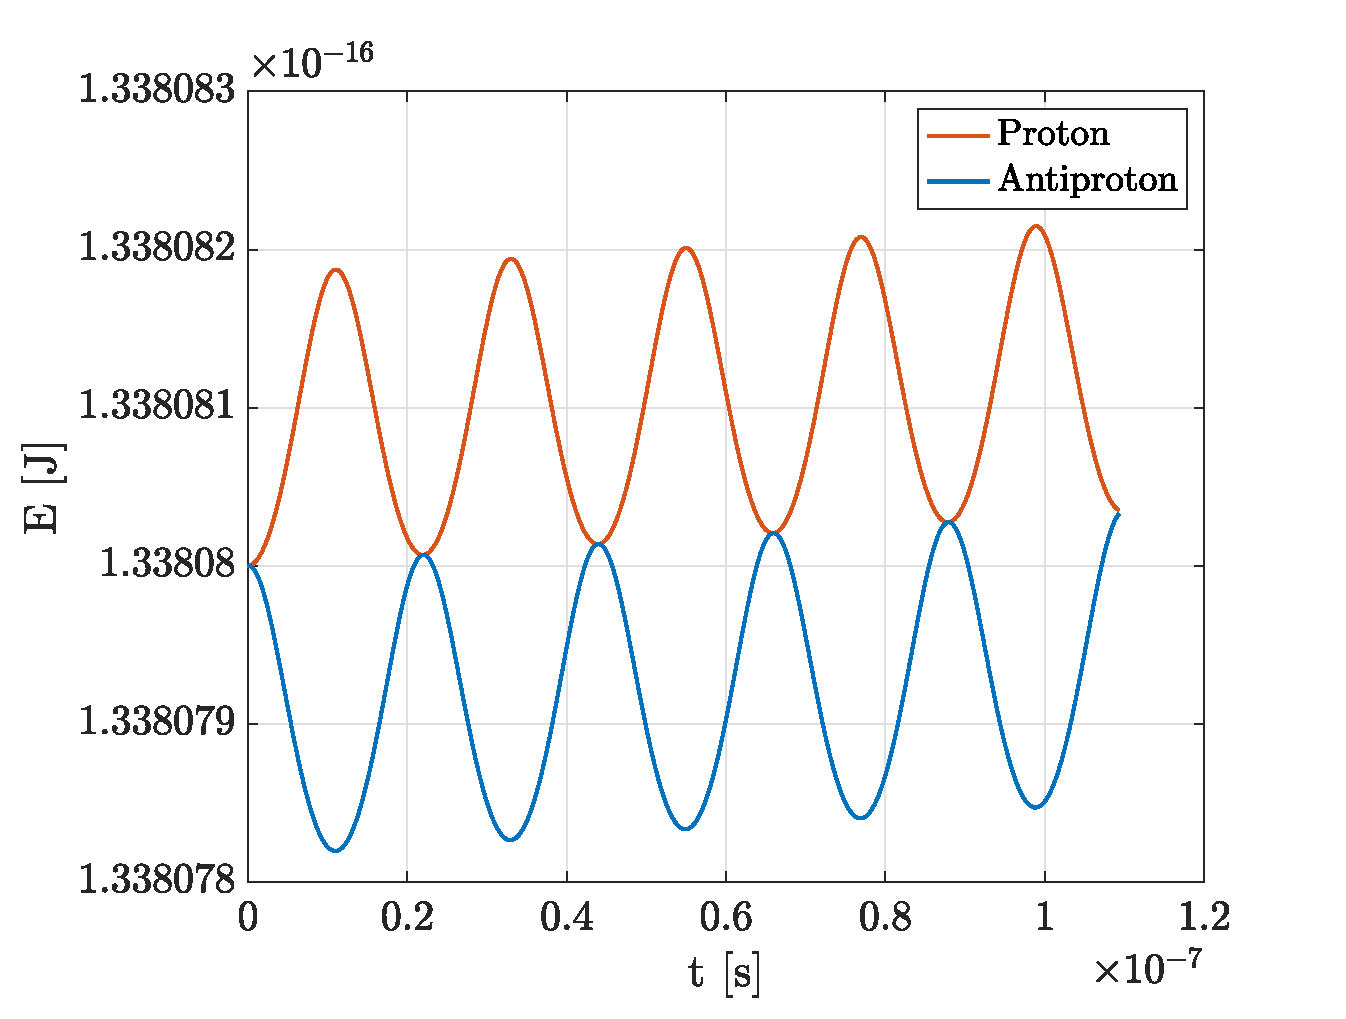
\includegraphics[width=0.75\textwidth]{graphs/app2_i_ene.eps}
	\caption{Comparison of the evolution of the energy for a proton and an antiproton in the magnetic field $\vec{B}$}
	\label{fig:app2_i_ene}
\end{figure}

On figure \ref{fig:app2_i_ene} the energy of the particles oscillates and increases on average, but the variation is infinitesimally small (of order $10^{22}$) and as such can be attributed to numerical error, as energy should be conserved.


\subsubsection{Magnetic moment $\mu$} %TODO Actually explain what the magnetic moment is

The magnetic moment is defined by:
\begin{equation}
\mu = \frac{mv^2}{2B} \si{\joule \per \tesla} = \frac{mv_0^2}{2B_0(1+\kappa x)} \si{\joule \per \tesla} = \frac{2.67616 \times 10^{-16}}{6+600x} \si{\joule \per \tesla}
\end{equation}
for a proton in the variable magnetic field $\vec{B}$.

\begin{figure}[h]
\centering
	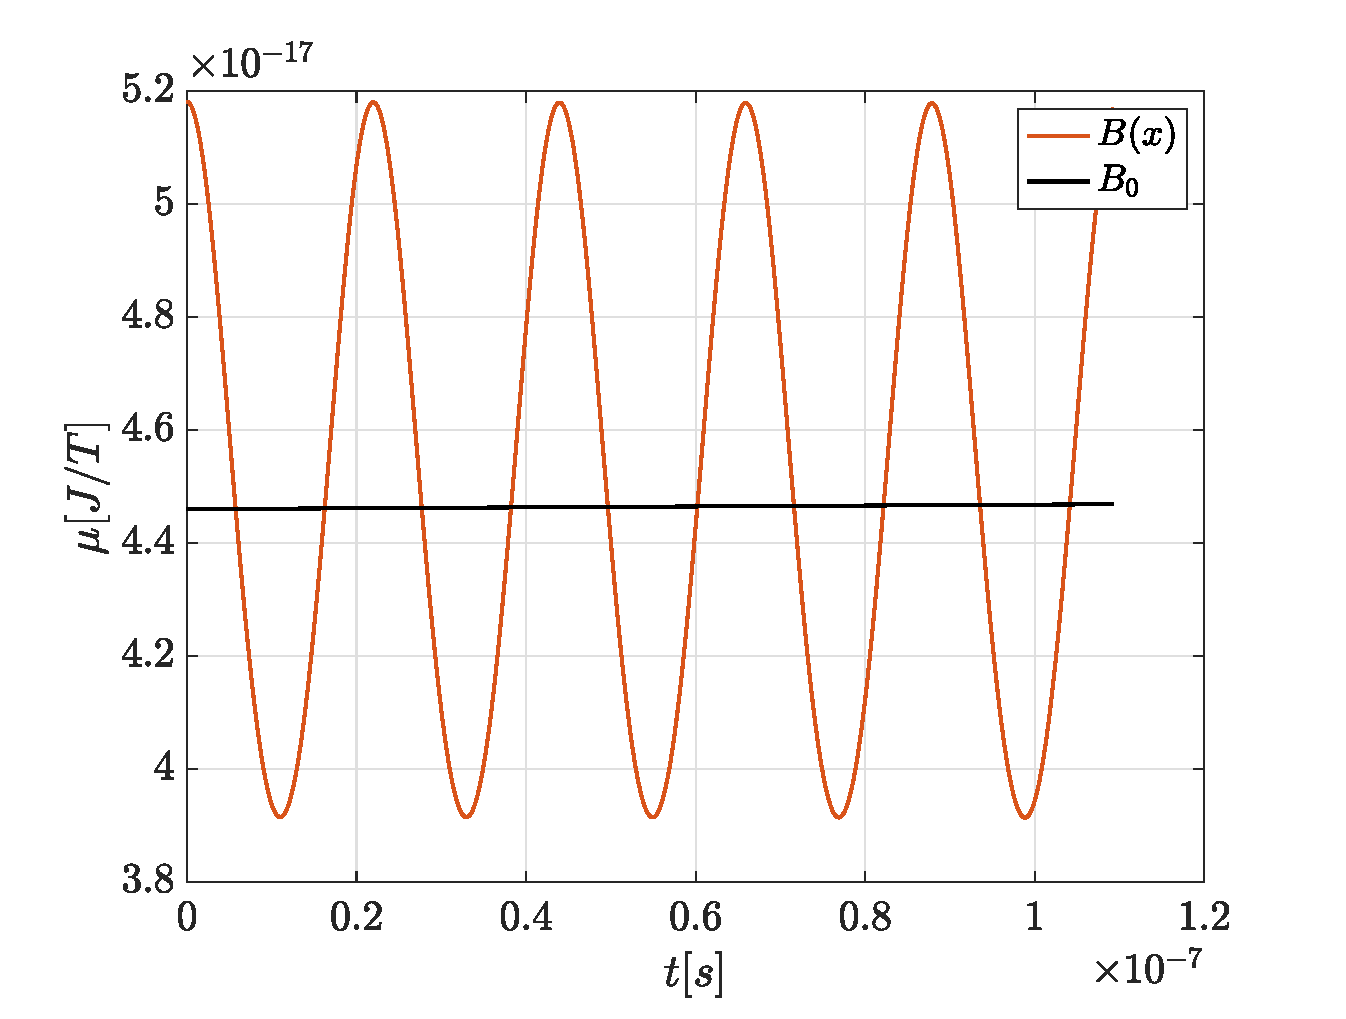
\includegraphics[width=0.60\textwidth]{graphs/mu.eps}
	\caption{Comparison of the magnetic moment $\mu$ for a proton in the variable magnetic field $B(x)\hat{z}$ and a proton in the constant magnetic field $B_0\hat{z}$}
	\label{fig:mu}
\end{figure}

The magnetic moment is defined as a vectorial quantity representing the intensity and the orientation of a source generating a magnetic field.\cite{wiki:magnetic-moment}
Figure \ref{fig:mu} shows a comparison between the magnetic moment of both the constant and variable magnetic fields.
The magnetic moment of the magnetic field $B_0$ is constant over time, which is correct with respect to the definition of the magnetic moment.
If the intensity of a magnetic field is constant, the magnetic moment will also be constant.
On the other hand, the magnetic moment of the variable magnetic field $\vec{B}(x)$ oscillates, which is also correct.
$\vec{B}(x)$ depends on the horizontal position of the proton, which also oscillates over time according to figure \ref{fig:app2-position}. 

\begin{figure}
\centering
	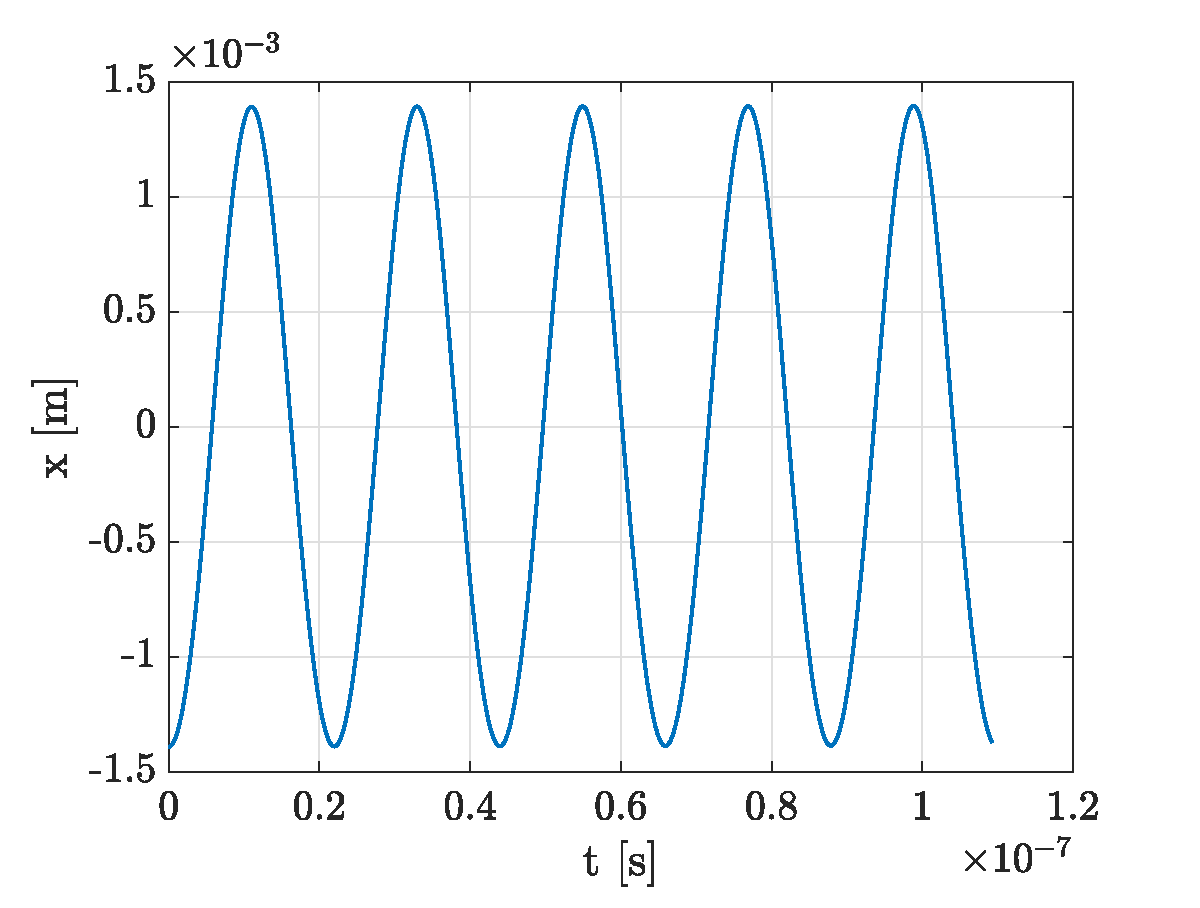
\includegraphics[width=0.6\textwidth]{graphs/app2_x.eps}
	\caption{Horizontal position of the proton with respect to time.}
	\label{fig:app2-position}
\end{figure}

\section{Conclusion}
The first few simulations showcased the differences between three integration methods and compared their respective stabilities, and it was concluded that the Runge-Kutta method of 2nd order was the best out of them.

It was observed that the trajectory of a proton in an electromagnetical field is influenced by whether the electrical field is null and whether the magnetic field is constant: in the case of a null electrical field and a constant magnetic field, its trajectory is circular. However when an electrical field is introduced, the trajectory becomes a spiral perpendicular to the electrical field, and when the magnetic field is variable, the trajectory becomes a spiral perpendicular to the magnetic field.

\appendix
\section*{Appendix}
\addcontentsline{toc}{section}{Annexes}

\section{Differential equation development} \label{ann:dev-eq-diff}
The mass of the proton is so small, that the gravitational force is ignored in these experiments.
Then the only force remaining is Lorentz's force.

\begin{equation*}
	\vec{F}_L = q(\vec{E} + \vec{v}\times\vec{B})
	\label{eq:lorentz-force}
\end{equation*}

Using Newton's second law, three equations results.

\begin{align*}
	\Sigma\vec{F}^{ext} &= m\vec{a} \\
	\vec{F}_L &= m\vec{a}\\
	q(\vec{E} + \vec{v}\times\vec{B}) &= m\vec{a} \\
	q\left( \begin{pmatrix} 0\\ E\\ 0\\ \end{pmatrix} + \begin{pmatrix} \dot{x}\\ \dot{y}\\ 0\\ \end{pmatrix} \times \begin{pmatrix} 0\\ 0\\ B\\ \end{pmatrix}\right) &= m\begin{pmatrix} \ddot{x}\\ \ddot{y}\\ \ddot{z}\\ \end{pmatrix} \\
	\frac{q}{m}\begin{pmatrix} B\dot{y}\\ E - B\dot{x}\\ 0 \end{pmatrix} &= \begin{pmatrix} \ddot{x}\\ \ddot{y}\\ \ddot{z}\\ \end{pmatrix}
\end{align*}

The last equation is not useful for what is about to come.
The system of differential equation resulting is equation \ref{eq:equa-diff}.

\section{Analytical solutions development} \label{ann:dev-sol-ana}
We solve the differential equation system \ref{eq:equa-diff-simple} for $v_x = \dot{x}$ and $v_y = \dot{y}$.

First, we set $\omega = \frac{qB_0}{m}$.

\begin{equation*}
	\begin{pmatrix} \dot{v_x}\\ \dot{v_y}\\ 0\\ \end{pmatrix} = \omega \begin{pmatrix} v_y\\ -v_x\\ 0\\ \end{pmatrix}
\end{equation*}

Then we derive the system with respect to time:

\begin{equation*}
	\begin{pmatrix} \ddot{v_x}\\ \ddot{v_y}\\ 0\\ \end{pmatrix} = \omega \begin{pmatrix} \dot{v_y}\\ -\dot{v_x}\\ 0\\ \end{pmatrix} = -\omega ^2 \begin{pmatrix} v_x\\ v_y\\ 0\\ \end{pmatrix}
\end{equation*}

Which gives us the differential equation for a harmonic oscillator. Thus we use the ansatz:

\begin{equation*}
	\begin{pmatrix} v_x\\ v_y\\ 0\\ \end{pmatrix} = \begin{pmatrix} Acos(\omega t + \phi_x)\\ Bcos(\omega t + \phi_y)\\ 0\\ \end{pmatrix}
\end{equation*}
with $A$, $B$ the amplitudes and $\phi_x$, $\phi_y$ the phases.

Thus we have: $\dot{vy} = -\omega v_x = -A \omega cos (\omega t + \phi_x)$. By integrating this result we get the solution shown in equation \ref{eq:sol-ana}:

\begin{equation*}
	\begin{pmatrix} v_x\\ v_y\\ 0\\ \end{pmatrix} = \begin{pmatrix} Acos(\omega t + \phi_x)\\ -Asin(\omega t + \phi_x)\\ 0\\ \end{pmatrix}
\end{equation*}

And with the initial conditions $v_{x0}=0$, $v_{y0}=v_0$:

\begin{equation*}
	\begin{pmatrix} 0\\ v_0\\ 0\\ \end{pmatrix} = \begin{pmatrix} Acos(\phi_x)\\ -Asin(\phi_x)\\ 0\\ \end{pmatrix}
\end{equation*}

Therefore $\phi_x = -\pi /2$ and $A=v_0$, and we get:

\begin{equation*}
	\begin{pmatrix} v_x\\ v_y\\ 0\\ \end{pmatrix} = \begin{pmatrix} v_0 sin(\omega t)\\ -v_0 cos(\omega t)\\ 0\\ \end{pmatrix}
\end{equation*}
which, by integrating and derivating, respectively, gives us the acceleration and trajectory vectors for a trajectory centered on $(0,0)$:

\begin{equation*}
	\begin{pmatrix} a_x\\ a_y\\ 0\\ \end{pmatrix} = \begin{pmatrix} v_0 \omega cos(\omega t)\\ v_0 \omega sin(\omega t)\\ 0\\ \end{pmatrix}
\end{equation*}

\begin{equation*}
	\begin{pmatrix} x\\ y\\ 0\\ \end{pmatrix} = \begin{pmatrix} -\frac{v_0}{\omega} cos(\omega t)\\ -\frac{v_0}{\omega} sin(\omega t)\\ 0\\ \end{pmatrix}
\end{equation*}

	Thus we get:

\begin{equation*}
	\begin{pmatrix} x_0\\ y_0\\ 0\\ \end{pmatrix} = \begin{pmatrix} -\frac{v_0}{\omega}\\ 0\\ 0\\ \end{pmatrix}
\end{equation*}
as the particle's initial position.


\begin{thebibliography}{99}
	\bibitem{wiki:magnetic-moment}
	Wikipedia contributors. (2018, September 3). Magnetic moment. In Wikipedia, The Free Encyclopedia. Retrieved 15:59, October 22, 2018, from \url{https://en.wikipedia.org/w/index.php?title=Magnetic_moment&oldid=857904512}
\end{thebibliography}

\end{document}
